\documentclass[xcolor=table, handout]{beamer}

\usepackage{shyne}

% Theme settings
\setbeamertemplate{navigation symbols}{}

\usetheme{Madrid}
\usefonttheme{structurebold}
\usefonttheme[onlymath]{serif}

\AtBeginSection[]
{ 	\begin{frame}{}

	{
	\usebeamerfont{frametitle}
	\begin{beamercolorbox}
		[wd={\textwidth}, center, sep=.2in, rounded=true, shadow=true]
		{frametitle}
	Chapter \thesection\\  \secname 
	\end{beamercolorbox}
	}
	
	\end{frame} 
}

\AtBeginSubsection[]
{ 	\begin{frame}{}

	{
	\usebeamerfont{frametitle}
	\begin{beamercolorbox}
		[wd={\textwidth}, center, sep=.2in, rounded=true, shadow=true]
		{frametitle}
	Section \thesection .\thesubsection\\  \subsecname 
	\end{beamercolorbox}
	}
	
	\end{frame} 
}

\title[Chapter 9]{Stat 201: Statistics I\\ Chapter 9 }
\author[M. Shyne]{}
\institute[Metro State]{
\includegraphics[width=1.75in]{../images/metro_logo}}
\date[5/9/2018]{
\\ \bigskip \bigskip 
\includegraphics[width=.4in]{../images/cc_big}}


\begin{document}
\frame{\titlepage}

% Chapter 9
\setcounter{section}{8}
\section{Inferences from Two Samples}

\begin{frame}{Two sample hypothesis testing}
\begin{block}{}
\large
Previously, a single sample was used to test whether the population from which the sample was drawn was the same or similar to a known population. More precisely, an hypothesis test compares an unknown population parameter to a known value.\\
\pause\medskip
Hypothesis testing can be used to compare two unknown populations using samples drawn from each population. This is unsurprisingly known as \bt{two sample hypothesis testing}. These tests compare two unknown population parameters.
\end{block}
\end{frame}

\begin{frame}{Null hypotheses}
\begin{block}{}
\large
Recall, to conduct an hypothesis test, two hypotheses are declared, the null hypothesis and the alternative hypothesis.\\
\end{block}

\pause
\begin{block}{}
\large
The null hypothesis is the claim that nothing interesting has occurred. For one sample tests, the null hypothesis states that the unknown population parameter is the same as the known parameter or some other known value.\\
\medskip
\pause For two sample tests, the null hypothesis states that the two unknown parameters are the same.\\
\medskip
\pause For example, if comparing means, $H_0: \mu_1 = \mu_2$, or the mean of population 1 is the same as the mean of population 2.
\end{block}
\end{frame}

\begin{frame}{Alternative hypotheses}
\begin{block}{}
\large
The alternative hypothesis is then the claim that something interesting has occurred. For one sample tests, the alternative hypothesis states that the unknown population parameter is somehow different from the known parameter. The unknown parameter might be less than, greater than or simple not equal to the known value. \\
\pause\medskip
For two sample tests, the alternative hypothesis states that the two unknown parameters are different. Similar to a one sample test, the alternative hypothesis could state that the first population parameter is less than, greater than or not equal to the second population parameter.\\
\pause\medskip
For example, if comparing means, $H_a: \mu_1 < \mu_2$ or $\mu_1 > \mu_2$ or $\mu_1 \ne \mu_2$.
\end{block}
\end{frame}

\begin{frame}{Conducting two sample hypothesis test}
\begin{block}{}
\large
Once the null and alternative hypotheses are determined, two sample hypothesis tests are carried out almost identically to one sample hypothesis tests.\\
\medskip
Assuming the null hypothesis is true, a test statistic representing the place of the samples within the appropriate sampling distribution is calculated. A p-value representing the probability of obtaining the test statistic or one more extreme is calculated. If the p-value is below a pre-determined threshold (the significance level), then the null hypothesis is rejected and it can be said that there is evidence for the alternative hypothesis.
\end{block}
\end{frame}

\begin{frame}{Steps for hypothesis test}
\begin{block}{}
\large
\begin{enumerate}
\item Identify null and alternative hypotheses from research question
\item Determine appropriate sampling distribution
\item Calculate test statistic
\item Calculate p-value
\item Compare p-value to significance level $\alpha$ and report decision
\item State conclusion in terms of original research question
\end{enumerate}
\end{block}
\end{frame}

\begin{frame}{Confidence intervals as hypothesis test}
\begin{block}{}
\large
Recall, a confidence interval can be used as an equivalent to a hypothesis test with the area outside the interval as rejection region. For two-sided tests, given a $(1-\alpha)$\% confidence interval, reject the null if the null parameter is outside of the interval.  
\end{block}
\medskip
{\centering
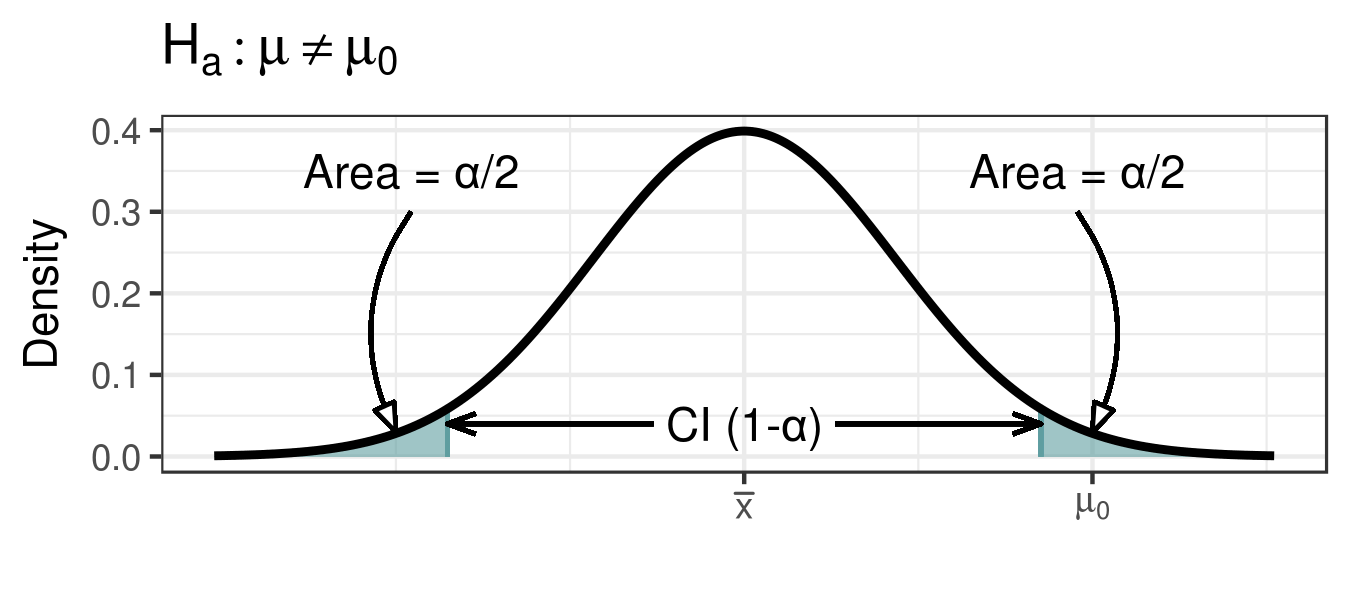
\includegraphics[width=4.5in]{../images/ch09_two_ci}
\par}
\end{frame}

\begin{frame}{Confidence intervals for one-sided tests}
\begin{block}{}
\large
However, for one-sided tests the rejection region is only on one side of the distribution. Thus, to get a one-sided rejection region with area $\alpha$ a $(1-2\alpha)$\% confidence interval is needed.
\end{block}
\medskip
{\centering
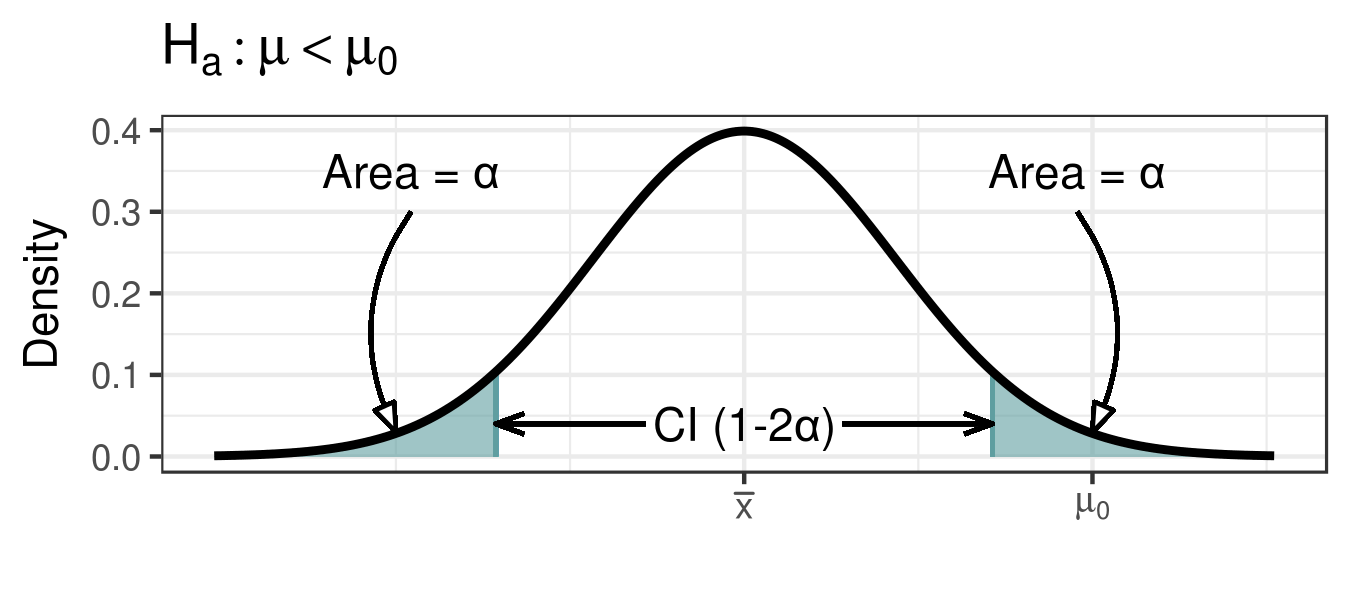
\includegraphics[width=4.5in]{../images/ch09_one_ci}
\par}
\end{frame}


% Section 9.1
\subsection{Two Proportions}

\begin{frame}{Two sample hypothesis tests for proportions}
\begin{block}{}
\large
A two sample hypothesis test can be conducted to compare the proportions of two populations.\\
\pause\medskip
Notationally, $p_1$ is the population proportion from the first population and $p_2$ is the population proportion from the second population. Similarly, $\hat p_1 = x_1/n_1$, the sample proportion of the sample from the first population is the number of successes in sample 1 divided by the sample size of sample 1, etc.\\
\pause\medskip
It is usually not important which of the two populations is ``first", but it is very important that which ever designation is used, it is used consistently through the hypothesis test process.
\end{block}
\end{frame}

\begin{frame}{Requirements}
\begin{block}{}
\large
\begin{itemize}
\item Both samples must meet the requirements of a binomial distribution (simple random samples, consistent probability of success for each trial, etc.)
\pause\item For each sample, the number of successes and the number of failures must both be 5 or greater.
\end{itemize}
\end{block}
\end{frame}


\begin{frame}{Null hypotheses}
\begin{block}{}
\large
The null hypothesis for a two sample proportion test is \emph{always} proportion 1 is equal to proportion 2, or\\
\smallskip
{\centering $H_0: p_1 = p_2$ \par}
\pause\medskip
However, the null hypothesis can be rewritten, without changing it's meaning, as\\
\smallskip
{\centering $H_0: p_1 - p_2 = 0$ \par}
\pause\medskip
This second representation more accurately depicts how the hypothesis is conducted and it is the representation used by StatCrunch. In most circumstances, either can be used.
\end{block}
\pause
\begin{block}{}
\large
Thus, under the null hypothesis, the two population proportions are the same and the common proportion can be estimated by\\
\medskip
{\centering
$\ds \bar p = \frac{x_1 + x_2}{n_1 + n_2}$
\par}
\end{block}
\end{frame}

\begin{frame}{Alternative hypotheses}
\begin{block}{}
\large
The alternative hypothesis for a two sample proportion test is that proportion 1 differs from proportion 2. Like one sample tests, two sample alternative hypotheses can be one-sided or two-sided. And like the null hypothesis for two sample tests, each alternative hypothesis can be written in two ways.\\
\smallskip
{\centering 
\begin{tabular}{r c | c}
Less than: & $H_a: p_1 < p_2$ & $H_a: p_1 - p_2 < 0$\\
Greater than: & $H_a: p_1 > p_2$ & $H_a: p_1 - p_2 > 0$\\
Not equal: & $H_a: p_1 \ne p_2$ & $H_a: p_1 - p_2 \ne 0$
\end{tabular}
\par}

\end{block}
\end{frame}

\begin{frame}{Test statistic}
\begin{block}{}
\large
Like with one sample proportion tests, two sample proportion tests use the standard normal sampling distribution. As always, z-scores are calculated by\\
\medskip
{\centering $\ds z = \frac{x - \mu}{\sigma}$ \par}
\pause\medskip
In this case, 
\begin{itemize}
\pause\item $x$ is the difference of the sample proportions, or $\hat p_1 - \hat p_2$
\pause\item the expected value is the difference of the population proportions, or $p_1 - p_2$, which under the null is 0
\pause\item $\sigma$ (standard deviation) is... complicated...\\
\medskip
{\centering $\ds \sigma = \sqrt{(\bar p \bar q)\Paren{\frac {1}{n_1} + \frac {1}{n_2}}}$
\par}
\medskip
\end{itemize}
\end{block}
\end{frame}

\begin{frame}{Test statistic, cont.}
\begin{block}{}
\large
The test statistic for two sample proportion tests is\\
\medskip
{\centering $\ds z = \frac{\hat p_1 - \hat p_2}{\sqrt{(\bar p \bar q)\Paren{1/n_1 + 1/n_2}}}$ \par}
\medskip
As before, z-scores and p-values can be found using technology.
\end{block}
\end{frame}

\begin{frame}{Hypothesis tests for two proportions in StatCrunch}

\begin{block}{}
\begin{itemize}
\large
\item Stat $\to$ Proportion Stats $\to$ Two Samples $\to$ With Summary
\item Enter ``\# of successes" and ``\# of observations" for sample 1 and sample 2
\item Select ``Hypothesis test for $p_1 - p_2$"
\item The null hypothesis should always be $H_0: p_1 - p_2 = 0$
\item Enter the appropriate value for the alternative hypothesis.
\item Click ``Compute!"
\item The test statistic and p-value are found in ``Z-Stat" and ``P-value"
\end{itemize}
\end{block}

\end{frame}

\begin{frame}{Confidence interval for difference of proportions}
\begin{block}{}
\large
\begin{itemize}
\item A confidence interval for the difference of population proportions $p_1 - p_2$, is defined as\\
\smallskip
{\centering $\ds CI_{1-\alpha} = (\hat p_1 - \hat p_2) \pm z_{\alpha/2} \sqrt{\frac {\hat p_1 \hat q_1}{n_1} + \frac {\hat p_2 \hat q_2}{n_2}}$ \par}
\smallskip
\pause\item A confidence interval that does not contain zero is evidence that the population proportions are not equal.

\pause\item Because hypothesis tests and confidence intervals use different estimates for standard deviation, it is possible to get different results.

\pause\item Remember, for one-sided tests, construct a $(1-2\alpha)$\% confidence interval.
\end{itemize}
\end{block}
\end{frame}




\begin{frame}{Confidence intervals for difference of proportions in StatCrunch}

\begin{block}{}
\begin{itemize}
\item Stat $\to$ Proportion Stats $\to$ Two Samples $\to$ With Summary
\item Enter ``\# of successes" and ``\# of observations" for sample 1 and sample 2
\item Select ``Confidence interval for $p_1 - p_2$"
\item Enter the appropriate confidence level.
\item Click ``Compute!"
\item The confidence interval bounds are found in ``L. Limit" and\\ ``U. Limit"
\end{itemize}
\end{block}

\end{frame}

\begin{frame}{Hypothesis test for two proportions, example}
\begin{exampleblock}{Example}
\large
A school district in an effort to reduce the number of teen drivers who text or email while driving creates an education program that half the high school students in the district attend. Two months after the program, the district surveys a random sample of teen drivers. The survey finds that 62 out of 212 teens surveyed who had attended the program (population 1) had texted or emailed while driving during the previous month, while among those that did not attend the program (population 2), 59 out of 173 did so.\\
\medskip
Test whether the program had an effect at 0.05 level of significance.
\begin{enumerate}
\pause\item Identify null and alternative hypotheses from research question\\
\pause$H_0: p_1 = p_2$ or $H_0: p_1 - p_2 = 0$\\
$H_a: p_1 \ne p_2$ or $H_a: p_1 - p_2 \ne 0$\\
\end{enumerate}
\end{exampleblock}
\end{frame}

\begin{frame}{Hypothesis test for two proportions, example}
\begin{exampleblock}{Example}
\large
\begin{enumerate}
\setcounter{enumi}{1}
\item Check the requirements for using normal distribution
\pause\begin{itemize}
\item Simple random sample
\item Requirements of a binomial satisfied (fixed sample size, two outcomes, independent, constant probability of success)
\item Successes and failures from both samples exceed 5
\end{itemize}
\pause\item Calculate $z$ test statistic\\
\pause$z = -1.0215331$
\pause\item Calculate p-value\\
\pause$p = 0.307$
\end{enumerate}
\end{exampleblock}
\end{frame}

\begin{frame}{Hypothesis test for a proportion, example}
\begin{exampleblock}{Example}
\large
\begin{enumerate}
\setcounter{enumi}{4}
\item Compare p-value to significance level $\alpha$ and report decision\\
\pause$p = 0.307 > \alpha =0.05$. Fail to reject null hypothesis.

\pause\item State conclusion in terms of original research question\\
\pause There is not evidence that teen drivers who attended the program text and email while driving at a different rate than those who did not attend.\\
{\centering or \par}\smallskip
There is not evidence that the education program changed the rates of teen drivers texting or emailing while driving.
\end{enumerate}

\end{exampleblock}
\end{frame}

\begin{frame}{Confidence interval for two means, example}
\begin{exampleblock}{Example}
\large
A ($1-\alpha$)\%, or 95\%, confidence interval for $p_1 - p_2$ is\\
\pause\medskip
{\centering $\ds CI_{0.95} = (-0.142, \, 0.045)$ \par}
\medskip

\pause Since zero is in the interval, there is not evidence that $p_1 - p_2 \ne 0$ or that teen drivers who attended the program text and email while driving at a different rate than those who did not attend.

\end{exampleblock}
\end{frame}

\begin{frame}<handout:0>{Group work}
\begin{block}{}
\large
\begin{itemize}
\item Complete question 1
\end{itemize}
\end{block}
\end{frame}


% Section 9.2
\subsection{Two Means: Independent Samples}

\begin{frame}{Two sample hypothesis tests for means}
\begin{block}{}
\large
A two sample hypothesis test can be conducted to compare the means of two populations.\\
\pause\medskip
Similar to proportion tests, parameters and statistics are designated with subscripts to identify which populations or samples they are from, $\mu_1$ and $\mu_2$, etc.
\end{block}
\end{frame}

\begin{frame}{Independent vs. dependent samples}
\begin{block}{}
\large
Before conducting a test, it must be determined whether the samples are independent or dependent.\\
\pause\medskip
\bt{Independent samples} are samples that come from distinct populations where the values from one sample do not affect the values from the other samples.\\
\pause\medskip
Conversely, \bt{dependent samples} are samples that often involve the same subjects with measurements taken at different times.
\end{block}
\end{frame}

\begin{frame}{Independent vs dependent samples, example}
\begin{exampleblock}{Example}
\large
Independent samples:
\begin{itemize}
\item Scores on statistic final in one class vs another class
\item Heights of men vs heights of women
\item In a clinical trial, outcomes for patients given experiment treatment vs patients given placebo (control)
\end{itemize}
\pause
Dependent samples:
\begin{itemize}
\item Scores on midterm exam vs final exam
\item Heights of husbands vs heights of wives
\item In a case control study, risk factors for subjects with disease vs matched subjects without disease
\end{itemize}
\end{exampleblock}
\end{frame}

\begin{frame}{Null and alternative hypotheses}
\begin{block}{}
\large
Similar to two sample proportion tests, the null hypothesis for two sample mean tests is always $H_0: \mu_1 = \mu_2$ or $H_0: \mu_1 -\mu_2 = 0$.\\
\medskip
Alternative hypotheses can be any of\\
\medskip
{\centering $H_a: \mu_1 < \mu_2, \, \mu_1 > \mu_2, \, \mu_1 \ne \mu_2$ \par}
\medskip
 or the equivalent forms of \\
 \medskip
{\centering $H_a: \mu_1 - \mu_2 < 0, \, \mu_1 - \mu_2 > 0, \, \mu_1 - \mu_2 \ne 0$ \par}
\medskip

\end{block}
\end{frame}

\begin{frame}{Requirements}
\begin{block}{}
\large
Both samples must be independent and simple random samples drawn from normal populations or have a sample size of at least 30.
\end{block}
\end{frame}

\begin{frame}{Test statistic}
\begin{block}{}
\large
As with one sample mean tests, two sample mean tests use a t distribution. Similar to two sample proportion tests, a t statistic  is calculated by\\
\medskip
{\centering $\ds t = \frac {\bar x_1 - \bar x_2}{\sqrt{\frac{s_1^2}{n_1} + \frac{s_2^2}{n_2}}}$ \par}
\medskip\pause
Recall, the degrees of freedom of a t distribution is defined by sample size minus one ($n-1$). For a two sample test, a conservative approach is to use the smaller of the degrees of freedom from the two samples.\\
\medskip
{\centering $\ds df = \min\Brack{(n_1-1) , (n_2-1)}$ \par}
\pause\medskip
When using technology, a more complicated, but accurate value will be used for the degrees of freedom.
\end{block}
\end{frame}

\begin{frame}{Hypothesis tests for two means in StatCrunch}

\begin{block}{}
\large
\begin{itemize}
\item Stat $\to$ T Stats $\to$ Two Samples $\to$ With Summary
\item Enter ``Sample mean", ``Sample std. dev." and ``Sample size" for both samples
\item Leave ``Pool variances" unchecked
\item Select ``Hypothesis test for $\mu_1 - \mu_2$"
\item The null hypothesis should always be $H_0: \mu_1 - \mu_2 = 0$
\item Enter the appropriate value for the alternative hypothesis.
\item Click ``Compute!"
\item The test statistic and p-value are found in ``T-Stat" and ``P-value"
\end{itemize}
\end{block}

\end{frame}

\begin{frame}{Confidence intervals for difference of means in StatCrunch}

\begin{block}{}
\large
\begin{itemize}
\item Stat $\to$ T Stats $\to$ Two Samples $\to$ With Summary
\item Enter ``Sample mean", ``Sample std. dev." and ``Sample size" for both samples
\item Leave ``Pool variances" unchecked
\item Select ``Confidence interval for $\mu_1 - \mu_2$"
\item Enter the appropriate confidence level.
\item Click ``Compute!"
\item The confidence interval bounds are found in ``L. Limit" and\\ ``U. Limit"
\end{itemize}
\end{block}

\end{frame}

\begin{frame}{Hypothesis test for two means, example}
\begin{exampleblock}{Example}
\large
A study is conducted of the heights of Metro State students. The heights of a sample of 32 male students taking statistics (population 1) have a mean of $\bar x = 70.1$ with a standard deviation of $s=3.5$. The heights of a sample of 38 male students taking accounting (population 2) have a mean of $\bar x = 67.9$ with a standard deviation of $s=3.1$.\\
\medskip
Conduct a test at $\alpha=0.05$ level of significance of the claim that statistics students are taller than accounting students.
\begin{enumerate}
\pause\item Identify null and alternative hypotheses from research question\\
\pause$H_0: \mu_1 = \mu_2$ of $H_0: \mu_1 - \mu_2 = 0$\\
$H_a: \mu_1 > \mu_2$ or $H_a: \mu_1 - \mu_2 > 0$\\
\end{enumerate}
\end{exampleblock}
\end{frame}

\begin{frame}{Hypothesis test for two means, example}
\begin{exampleblock}{Example}
\large
\begin{enumerate}
\setcounter{enumi}{1}

\item Use a t distribution
\pause\item Calculate $t$ test statistic\\
\pause$t=2.7592694$
\pause\item Calculate p-value\\
\pause$p = 0.0038$
\pause\item Compare p-value to significance level $\alpha$ and report decision\\
\pause$p = 0.0038 < \alpha = 0.05$. Reject the null hypothesis.
\pause\item State conclusion in terms of original research question\\
\pause There is evidence that male statistics students are taller than male accounting students.
\end{enumerate}

\end{exampleblock}
\end{frame}

\begin{frame}{Confidence interval for two means, example}
\begin{exampleblock}{Example}
\large
A $(1-2\alpha)$\%, or 90\%, confidence interval for $\mu_1 - \mu_2$ is\\
\pause\medskip
{\centering $\ds CI_{0.90} = (0.869, \, 3.531)$ \par}
\medskip

\pause Since zero is not in the interval and both bounds are positive, there is evidence that $\mu_1 - \mu_2 > 0$ or male statistics students are taller than male accounting students.

\end{exampleblock}
\end{frame}

\begin{frame}<handout:0>{Group work}
\begin{block}{}
\large
\begin{itemize}
\item Complete question 2
\end{itemize}
\end{block}
\end{frame}

% Section 9.3
\subsection{Two Dependent Samples (Matched Pairs)}

\begin{frame}{Hypothesis tests for dependent samples}
\begin{block}{}
\large
Conceptually, when working with two dependent samples, also known as matched pairs, a new value $d = x_1 - x_2$ is calculated for each pair. Then, the null hypothesis $H_0: \mu_1 = \mu_2$ becomes $H_0: \mu_D = 0$ and the test is essentially a one sample hypothesis test for the mean of $d$.\\
\pause\medskip
Matched pairs tests, when appropriate, are preferable to independent samples tests because the variability between subjects is almost eliminated. Thus, the total variability is reduced resulting in a more accurate test. 
\end{block}
\end{frame}

\begin{frame}{Conducting a dependent samples test}
\begin{block}{}
\large
Since a dependent samples test is essentially a one sample test of the sample of difference values $d$, null and alternative hypotheses should be stated in terms of $\mu_D$ the population mean of the differences.\\
\pause\medskip
For example, $H_0: \mu_D = 0$ and $H_a: \mu_D < 0$.\\
\pause\medskip
The test statistic is calculated as a one sample statistic from the sample of differences\\
\medskip
{\centering $\ds t = \frac {\bar d}{\frac{s_d^2}{\sqrt{n}}}$ \par}
\medskip
\end{block}
\end{frame}

\begin{frame}{Hypothesis tests for matched pairs in StatCrunch}

\begin{block}{}
\large
\begin{itemize}
\item Stat $\to$ T Stats $\to$ Paired
\item Select columns of data for both samples
\item Select ``Hypothesis test for $\mu_D = \mu_1 - \mu_2$"
\item The null hypothesis should always be $H_0: \mu_D = 0$
\item Enter the appropriate value for the alternative hypothesis.
\item Click ``Compute!"
\item The test statistic and p-value are found in ``T-Stat" and ``P-value"
\end{itemize}
\end{block}

\end{frame}

\begin{frame}{Confidence intervals for matched pairs in StatCrunch}

\begin{block}{}
\begin{itemize}
\large
\item Stat $\to$ T Stats $\to$ Paired
\item Select columns of data for both samples
\item Select ``Confidence interval for $\mu_D = \mu_1 - \mu_2$"
item Enter the appropriate confidence level.
\item Click ``Compute!"
\item The confidence interval bounds are found in ``L. Limit" and\\ ``U. Limit"
\end{itemize}
\end{block}

\end{frame}

\begin{frame}{Hypothesis test for matched pairs, example}
\large
\begin{exampleblock}{Example}
A study is conducted to see if statistics students change their scores from the midterm exam to the final exam. 42 students who took both exams are randomly selected. Their scores are found in the file ``scores.csv".\\
\medskip
Test at significance level of 0.01 whether scores changed between the midterm and the final.
\begin{enumerate}
\pause\item Identify null and alternative hypotheses from research question\\
\pause$H_0: \mu_D = 0$\\
$H_a: \mu_D \ne 0$\\
\end{enumerate}
\end{exampleblock}
\end{frame}

\begin{frame}{Hypothesis test for matched pairs, example}
\begin{exampleblock}{Example}
\large
\begin{enumerate}
\setcounter{enumi}{1}

\item Use a t distribution
\pause\item Calculate $t$ test statistic\\
\pause$t=-3.8176772$
\pause\item Calculate p-value\\
\pause$p = 0.0004$
\pause\item Compare p-value to significance level $\alpha$ and report decision\\
\pause$p = 0.0004 < \alpha = 0.01$. Reject the null hypothesis.
\pause\item State conclusion in terms of original research question\\
\pause There is evidence that statistics exam scores change from the midterm to the final.
\end{enumerate}

\end{exampleblock}
\end{frame}

\begin{frame}{Confidence interval for matched pairs, example}
\begin{exampleblock}{Example}
\large
A ($1-\alpha$)\%, or 99\%, confidence interval for $\mu_D$ is\\
\pause\medskip
{\centering $\ds CI_{0.99} = (-6.871, \, -1.177)$ \par}
\medskip

\pause Since zero is not in the interval, there is evidence that $\mu_d \ne 0$ or statistics exam scores change from the midterm to the final.

\end{exampleblock}
\end{frame}

\begin{frame}<handout:0>{Group work}
\begin{block}{}
\large
\begin{itemize}
\item Complete question 3
\end{itemize}
\end{block}
\end{frame}


\begin{frame}{Teaching the null hypothesis}
\smallskip
{\centering

\includegraphics[width=2 in]{../images/ch09_null_hypothesis}
\par}
\end{frame}
\end{document}